\title{Simulating Cantilever Partial Differential Equations}
\author{John Till}
\date{}

\documentclass[12pt]{article}

\usepackage[a4paper, margin=0.75in]{geometry}
\usepackage[colorlinks=true,urlcolor=blue]{hyperref}
\usepackage{amsmath,amssymb}
\usepackage{graphicx}

\usepackage{xcolor}
\definecolor{OffWhite}{rgb}{0.93,0.93,0.93}
\definecolor{QtCommentColor}{rgb}{0,0.5,0}
\definecolor{QtKeywordColor}{rgb}{0.5,0.5,0}
\definecolor{QtPurpleColor}{rgb}{0.5,0,0.5}
\definecolor{QtGlobal}{rgb}{0.808,0.361,0}
\definecolor{QtFunctionColor}{rgb}{0,0.404,0.486}

\usepackage[T1]{fontenc} %for upquotes in listings
\usepackage{textcomp} %for upquotes in listings
\usepackage{listings}
\lstset{
		language=C++,
		escapeinside={!-}{-!},
		upquote=true,
		%
		otherkeywords={Vector3d, DiagonalMatrix, VectorXd, Matrix3d, Map, MatrixXd, TimeManagerBdfAlpha, Vector6d, std
									UnitX, pow, inverse, transposeMultiply, segment, data, UnitZ, cross, hat_postmultiply,
									Zero, Identity, UnitY, cosseratRodOde, cosseratRodPDE, ode4, col, row, main, plot, solveLevenbergMarquardt,
									TimeBdfAlpha_SpaceEuler, euler, objFunc, block, clock, advanceTime, endl, playAnimation},
    morekeywords=[2]{Vector3d, DiagonalMatrix, VectorXd, Matrix3d, Map, MatrixXd, TimeManagerBdfAlpha, Vector6d, std},
		morekeywords=[3]{UnitX, UnitZ, pow, inverse, transposeMultiply, segment, data, cross, hat_postmultiply,
		                 Zero, Identity, UnitY, cosseratRodOde, cosseratRodPDE, ode4, col, row, main, plot, solveLevenbergMarquardt,
										TimeBdfAlpha_SpaceEuler, euler, objFunc, block, clock, advanceTime, endl, playAnimation},
    %
		frame = single,
		rulecolor=\color{black},
    tabsize=4, % tab space width
    showstringspaces=false, % don't mark spaces in strings
		%
		basicstyle=\footnotesize,%\color{QtIdentifier},
		backgroundcolor=\color{OffWhite},
    commentstyle=\color{QtCommentColor}, % comment color
    keywordstyle=\color{QtKeywordColor}, % keyword color
		keywordstyle=[2]{\color{QtPurpleColor}},
		keywordstyle=[3]{\color{QtFunctionColor}},
    stringstyle=\color{QtCommentColor} % string color
}

\begin{document}

\makeatletter
\renewcommand{\@maketitle}{
\newpage
\null
\vskip 2em
\begin{center}
{\LARGE \@title \par}
\end{center}
\par
} \makeatother

\maketitle

In this chapter the partial differential equations (PDEs) describing a dynamic Cosserat are simulated. The theoretical development is described in the paper ``Real-Time Dynamics of Soft and Continuum Robots based on Cosserat-Rod Models'', which is in press with IJRR.

We start by defining the simulation parameters:
\begin{lstlisting}
//Independent Parameters
const double E = 200e9;
const double G = 80e9;
const double rad = 0.001;
const double rho = 8000;
const Vector3d g = -9.81*Vector3d::UnitX();
const double L = 0.5;
const int N = 40; //Number of spatial points
const double dt = 2e-3; //Time step
const double alpha = -0.2; //Parameter for implicit time discretization
const double T = 25; //Total simulation time
const double initial_tip_mass = 0.02; //Weight for ICs, released at t0+
const double Bs = 0; //Shearing material damping
const double Be = 0; //Extension material damping
const double Bb = 0; //Bending material damping
const double Bt = 0; //Torsional material damping
\end{lstlisting}
Familiar static parameters make up about half of this list. $dt$ is the time step, which is set to 2 milliseconds. ``alpha'' is a parameter of the BDF-$\alpha$ time discretization which controls the numerical damping. The total simulation time is $T$. The tip mass of 20 grams is present when the initial conditions (ICs) are calculated and is removed at the start of the dynamic simulation. In the last four lines we define material damping parameters for each of the deformation modes.

With the independent parameters taken care of, we calculate the dependent parameters:
\begin{lstlisting}
//Dependent parameter calculations
static Vector3d F = initial_tip_mass*g;
const double c0 = TimeManagerBdfAlpha::getC0(dt,alpha);
const double A = pi*pow(rad,2);
const double I = pi*pow(rad,4)/4;
const DiagonalMatrix<double, 3> Kse = DiagonalMatrix<double, 3>(G*A,G*A,E*A);
const Vector3d Kse_e3(0, 0, E*A);
const DiagonalMatrix<double, 3> Kbt = DiagonalMatrix<double, 3>(E*I,E*I,G*2*I);
const DiagonalMatrix<double, 3> Kse_inv =
   DiagonalMatrix<double, 3>(G*A,G*A,E*A).inverse();
const DiagonalMatrix<double, 3> Kbt_inv =
   DiagonalMatrix<double, 3>(E*I,E*I,G*2*I).inverse();
const DiagonalMatrix<double, 3> rhoJ = rho*DiagonalMatrix<double, 3>(I, I, 2*I);
const DiagonalMatrix<double, 3> Bse(Bs, Bs, Be);
const DiagonalMatrix<double, 3> Bbt(Bb, Bb, Bt);
const DiagonalMatrix<double, 3> inv_of_Kse_c0Bse
   (1/(G*A + c0*Bs), 1/(G*A + c0*Bs), 1/(E*A + c0*Be));
const DiagonalMatrix<double, 3> inv_of_Kbt_c0Bbt
   (1/(E*I + c0*Bb), 1/(E*I + c0*Bb), 1/(G*2*I + c0*Bt));
const double rhoA = rho*A;
const Vector3d rhoAg = rho*A*g;
\end{lstlisting}
We use the ``TimeManagerBdfAlpha'' class to abstract the details of the BDF-$\alpha$ method. There are several similar dependent parameters because many of these terms are calculated globally here to avoid repeated calculations in the PDE function, for example ``rhoAg''.

We will need to set the initial conditions for the dynamic problem by solving the steady-state response to a tip weight. This requires solving a static BVP, so we define a function for the static Cosserat rod equations:
\begin{lstlisting}
//ODE describing elastic rod statics
void cosseratRodOde(VectorXd& y_s_out, Map<VectorXd> z_out, Map<VectorXd> y){
    //Unpack state vector
    Matrix3d R = Map<Matrix3d>(&y[3]);
    Map<Vector3d> n(&y[12]);
    Map<Vector3d> m(&y[15]);

    //Hard-coded constitutive law w/ no precurvature
    Vector3d v = Kse_inv*transposeMultiply(R,n); v(2) += 1;
    Vector3d u = Kbt_inv*transposeMultiply(R,m);

    //Refer to the state vector derivative by its components
    Map<Vector3d> p_s (&y_s_out[0]);
    Map<Matrix3d> R_s (&y_s_out[3]);
    Map<Vector3d> n_s (&y_s_out[12]);
    Map<Vector3d> m_s (&y_s_out[15]);
    Map<Vector3d> q_s (&y_s_out[18]);
    Map<Vector3d> w_s (&y_s_out[21]);

    //ODEs
    p_s = R*v;
    R_s = hat_postmultiply(R,u);
    n_s = -rhoAg;
    m_s = -p_s.cross(n);
    q_s = Vector3d::Zero();
    w_s = Vector3d::Zero();

    //Output argument for variables with time derivatives
    z_out << Vector6d::Zero(), v, u;
}
\end{lstlisting}
This is similar to functions we've written previously, but there are two differences. First, we include the local-frame velocity $\boldsymbol{q}$ and local-frame angular velocity $\boldsymbol{\omega}$ as part of the state, even though they are zero for the static problem. The rationale for including the dynamic terms here is that it simplifies our coding process to have the same state vector for both problems. The second difference is that there is a vector ``z\_out'' as an output argument. $\boldsymbol{Z}$ contains the variables which we are numerically differentiating, and we need to solve the initial conditions of $\boldsymbol{Z}$ in order to calculate the history terms $\boldsymbol{Z}\_h$ for the first time step of the dynamic problem.

\newpage \noindent
Now we write the main part of our program- the PDE function:
\begin{lstlisting}
//PDE semi-discretized in time describing elastic rod dynamics
void cosseratRodPDE(VectorXd& y_s_out, Map<VectorXd> z_out,
                    Map<VectorXd> y, Map<VectorXd> z_h){
    //Unpack state vector
    Matrix3d R = Map<Matrix3d>(&y[3]);
    Vector3d n = Map<Vector3d>(&y[12]);
    Vector3d m = Map<Vector3d>(&y[15]);
    Vector3d q = Map<Vector3d>(&y[18]);
    Vector3d w = Map<Vector3d>(&y[21]);

    //Unpack history terms
    Map<Vector3d> q_h (&z_h[0]);
    Map<Vector3d> w_h (&z_h[3]);
    Map<Vector3d> v_h (&z_h[6]);
    Map<Vector3d> u_h (&z_h[9]);

    Vector3d q_t = c0*q + q_h;
    Vector3d w_t = c0*w + w_h;

    //Material constitutive equation
    Vector3d v = inv_of_Kse_c0Bse*(transposeMultiply(R,n) + Kse_e3 - Bse*v_h);
    Vector3d u = inv_of_Kbt_c0Bbt*(transposeMultiply(R,m) - Bbt*u_h);
    Vector3d v_t = c0*v + v_h;
    Vector3d u_t = c0*u + u_h;

    //Pack state vector derivative
    Map<Vector3d> p_s (&y_s_out[0]);
    Map<Matrix3d> R_s (&y_s_out[3]);
    Map<Vector3d> n_s (&y_s_out[12]);
    Map<Vector3d> m_s (&y_s_out[15]);
    Map<Vector3d> q_s (&y_s_out[18]);
    Map<Vector3d> w_s (&y_s_out[21]);

    //ODEs
    p_s = R*v;
    R_s = hat_postmultiply(R,u);
    n_s = rhoA*R*(q_t + w.cross(q)) - rhoAg;
    m_s = R*(rhoJ*w_t + w.cross(rhoJ*w)) - p_s.cross(n);
    q_s = v_t - u.cross(q) + w.cross(v);
    w_s = u_t - u.cross(w);

    //Output argument for variables with time derivatives
    z_out << q, w, v, u;
}
\end{lstlisting}
This implements the semi-discretized dynamic Cosserat rod equations as described in the paper. Once again we calculate and store $\boldsymbol{z}$ so that we can calculate $\boldsymbol{z}\_h$ at the next time step. We unpack the values of $\boldsymbol{z}\_h$ at this time step to calculate derivative terms in keeping with the time semi-discretization strategy.

Now we can declare the matrices which will define the rod's grid points.
\begin{lstlisting}
static MatrixXd Y(24,N); //State variables (which have arclength derivatives)
static MatrixXd Z(12,N); //Variables with time derivatives
static MatrixXd Z_h(12,N); //History terms
\end{lstlisting}

Finally we can write the objective function. Due to the similarities of the dynamic problem and the initial condition static problem, we write a single templated function which only differs in two places depending on which problem is being solved:

\begin{lstlisting}
template<bool is_dynamic>
VectorXd objFunc(VectorXd guess){
    VectorXd y0(24);
    y0 << 0, 0, 0, 1, 0, 0, 0, 1, 0, 0, 0, 1, guess, Vector6d::Zero();

    //Numerically integrate the semi-discretized rod PDEs
    if(is_dynamic) TimeBdfAlpha_SpaceEuler<cosseratRodPDE,24,12,N>(Y,Z,y0,L,Z_h);
    else           euler<cosseratRodOde,24,12,N>(Y,Z,y0,L);

    Vector3d nL_shooting = Y.block<3,1>(12, N-1);
    Vector3d mL_shooting = Y.block<3,1>(15, N-1);

    Vector6d distal_error;
    if(is_dynamic) distal_error << nL_shooting, mL_shooting; //No tip mass
    else distal_error << nL_shooting - F, mL_shooting; //Tip mass determines ICs

    return distal_error;
}
\end{lstlisting}
Depending on the template parameter, this will either integrate the static ODE or the semi-discretized dynamic PDE. The integration routines are defined in ``numericalpde.h''. After integrating, we determine how badly the equilibrium equations at the tip have been violated.

Now we have all the subfunctions we need and we can start on the main function. In the first step, we solve for the initial conditions:
\begin{lstlisting}
int main(int, char**){
    //Solve initial conditions
    Vector6d guess = Vector6d::Zero();
    Vector6d reaction_wrench = solveLevenbergMarquardt<objFunc<false> >(guess);
    TimeManagerBdfAlpha time_scheme(Z, Z_h, dt, alpha);
    F = Vector3d::Zero(); //The tip load is removed
\end{lstlisting}
We solve the static BVP subject to some attached tip mass, then we remove the tip mass. This has the side effect of setting $\boldsymbol{Z}$ to the correct initial value. After solving the static problem we create the time manager that will update the values of $\boldsymbol{Z}\_h$ at each time step.

With the ICs solved, we can tackle the PDE. In the next several lines we create the dynamic simulation loop:
\begin{lstlisting}
int M = static_cast<int>(T/dt);
MatrixXd px(M,N), pz(M,N);
std::!-\textcolor{QtPurpleColor}{clock\_t}-! start = std::clock();
for(int i = 0; i < M; i++){
		px.row(i) = Y.row(0);
		pz.row(i) = Y.row(2);
		time_scheme.advanceTime(); //Update Z_h from history of Z
		//Solve dynamic problem
		reaction_wrench=solveLevenbergMarquardt<objFunc<true> >(reaction_wrench);
}
double duration = ( std::clock() - start ) / static_cast<double>(CLOCKS_PER_SEC);
std::cout << "Time elasped: " << duration << "s" << std::endl;
std::cout << "Real-time ratio: " << T/duration << std::endl;
\end{lstlisting}
The two central lines are solving the problem and advancing the time. The time manager keeps track of the values of $\boldsymbol{Z}$ each time that ``advanceTime()'' is invoked so that it stores the state history needed for the derivative calculation. The class is defined in ``timemanagement.h''.

Besides solving the problem, we also time the simulation and store $\boldsymbol{p}_x$ and $\boldsymbol{p}_z$ at every time step so that we can create an animation of the dynamic cantilever response. Again our purpose is not to explore the details of plotting in Qt, so abstract the details with a function:
\begin{lstlisting}
#ifdef QT_CORE_LIB
playAnimation(pz, px, dt, "Dynamic Cantilever", "z (m)", "x (m)");
#endif
\end{lstlisting}
This is defined in ``simpleanimation.h''. Running the program will produce a window with an animation of the cantilever response.
\begin{figure}[h]
	\centering
		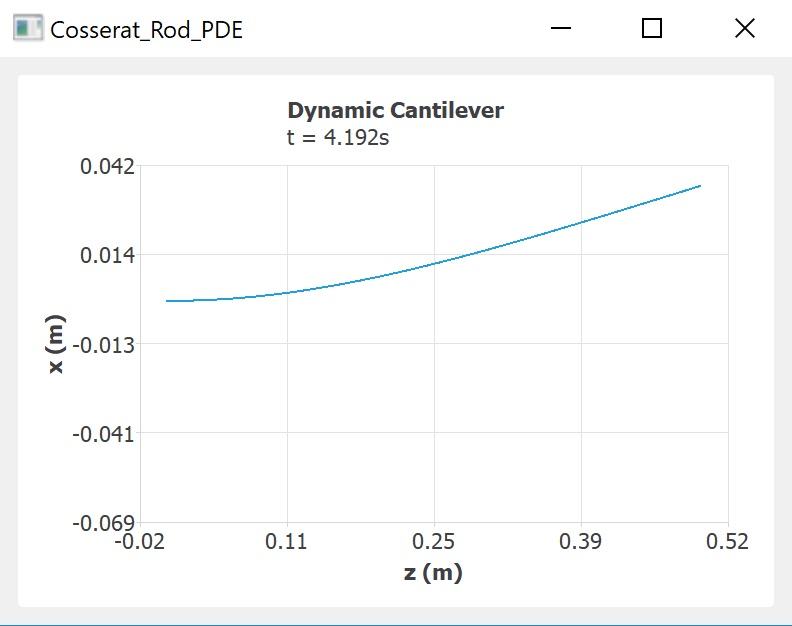
\includegraphics[width=0.7\textwidth]{fig/SolutionPlot.jpg}
	\label{fig:SolutionPlot}
\end{figure}

The Cosserat rod PDE problem is inherently complicated, but hopefully this code is terse and readable without too much sacrifice in performance. We could refactor the code and over-optimize our simulation by writing an integration method specifically for this set of PDEs. This is shown in the ``Cpp\_overoptimized'' folder, but is not discussed in detail here. The performance is about 2.5-3x better, but there is twice as much code and the integration routine is far too dense.

\end{document}